\section{State-of-the-art and Objectives}
%\noindent
\vspace{-4pt}

\subsection{Background}
\noindent
Quasars\footnote{ Historically, ``quasars'' and ``Active Galactic
Nuclei (AGN)'' have described different luminosity/classes of objects,
but here we use these terms interchangeably (with a preference for
quasar) in recognition of the fact that they both describe accreting
supermassive black holes \citep[e.g.][]{Haardt2016book}.}  are powered
by accretion of material onto supermassive black holes (SMBHs), via
accretion disks.  In the local Universe, there is a link between the
key properties of massive galaxies, such as bulge mass, and their
central supermassive black holes \citep[e.g., ][]{McLure_Dunlop2002,
HaringRix2004, Salviander2007, Greene2010, KormendyHo2013}. This has
led to the hypothesis that the supermassive black hole, when accreting,
has an influence on its host galaxy by the means of some regulatory
``feedback'' mechanism(s) \citep[e.g., ][]{Sijacki2007, Hopkins2008a,
AlexanderHickox2012, Fabian2012, KingPounds2015}. However, the details
of the physical processes involved in this `AGN/quasar feedback' are
still disputed and, moreover, direct observational evidence for quasar
feedback in the early universe is conspicuous by its absence
\citep[e.g., ][]{HeckmanBest2014, NaabOstriker2017}. Hence, a major
source of uncertainty in our current understanding of galaxy evolution
is how supermassive black holes influence, and potentially regulate,
their host galaxies \citep{Vogelsberger2013, Vogelsberger2014,
Schaye2015, Angles-Alcazar2013, Angles-Alcazar2017}.


\smallskip 
\smallskip
\noindent
Furthermore, the details of the physical processes involved in the
quasar activity including how the SMBH directly couples and affects
its most local environment, i.e., the accretion disk, broad line
region and dusty torus, are still unknown at this point
\citep[e.g.,][]{Netzer2015, Padovani2017}.

\smallskip 
\smallskip
\noindent
Although it has long been established that quasars are powered by
accretion discs surrounding supermassive black holes, there have also
been long-standing issues. For example, the observed spectral energy
distributions (SEDs) of typical quasars
\citep[e.g.,][]{Koratkar_Blaes1999, Sirko_Goodman2003} differ markedly
from classical predictions \citep[][]{SS73, Pringle1981} with a
typical observed quasar SED flat in $\lambda F_{\lambda}$ over several
decades in wavelength \citep{Elvis1994, Richards2006b}.  Also, real
accretion disks seem to be cooler \cite[e.g., ][]{Lawrence2012} and
larger \cite[e.g.,][]{Pooley2007, Morgan2010, Morgan2012,
Mosquera2011} than the standard accretion disk model predictions.

\smallskip 
\smallskip
\noindent
However, even more troubling are new observations of {\it extreme
variability} in some objects (see next section) - factors of several
over a decade or so, including, crucially, at optical wavelengths, and
not just in the extreme UV or in X-rays. This has led to the ``Quasar
Viscosity Crisis'' \citep{Lawrence2018}.

\smallskip 
\smallskip
\noindent
{\bf As such, we are left in the uncomfortable current situation of invoking
galaxy-wide ``quasar feedback'' in order to reconcile demographic
observations in cosmological-scale simulations, but where we currently
do not understand the physics of mechanism that is supposed to
initiate this necessary and vital energy transport.}


\subsubsection{Observational State-of-the-Art}
Here we present a concise overview of the observational
state-of-the-art in the brand new field of variable extragalactic
astrophysics, concentrating on quasar studies.

\smallskip
\smallskip
\noindent
\textbf{\textsc{A microscope for rapid Central Engines:}}
``Changing-look'' quasars \citep[CLQs; ][]{LaMassa2015,
Runnoe2016, Ruan2016, Runco2016, MacLeod2016, Yang2017} 
are defined to be luminous quasars which have a
dramatic appearance, or disappearance, of their broad emission-line
component on observed-frame month-to-year timescales.  CLQs are
important since they offer a direct observational probe into the
physical processes dictating the structure of the broad-line region
(BLR). These timescales can potentially be associated with the viscous
timescale (the drift time through the accretion disk), the light
crossing timescale (critical for reverberation mapping and disk
reprocessing) and the dynamical timescale of the BLR.  {\it CLQs are thus
an ideal laboratory for studying accretion physics, as the entire
system responds to a large change in ionizing flux on a human
timescale.}

\smallskip 
\smallskip
\noindent 
In \citet{MacLeod2016} I co-led the first systematic search for CLQs
based on photometry from SDSS and Pan-STARRS1, along with repeat
spectra from the SDSS/BOSS, and reported the discovery of 10
CLQs. This is a startling result since we now estimate
$\approx$10-15\% of bona fide quasars may exhibit `changing look'
behaviour on $\sim$10 year (rest-frame) timescales. However, plausible
time-scales for variable dust extinction are factors of $2-10$ too
long to explain the dimming and brightening in these sources.  Changes
in accretion rate are the currently favored explanation for CLQs, but
then the question of how the inner accretion disk couples to the BLR
immediately arises. Further investigation is thus warranted.

\begin{figure}[h]
  \begin{center}
    \hspace{-0.5cm}
    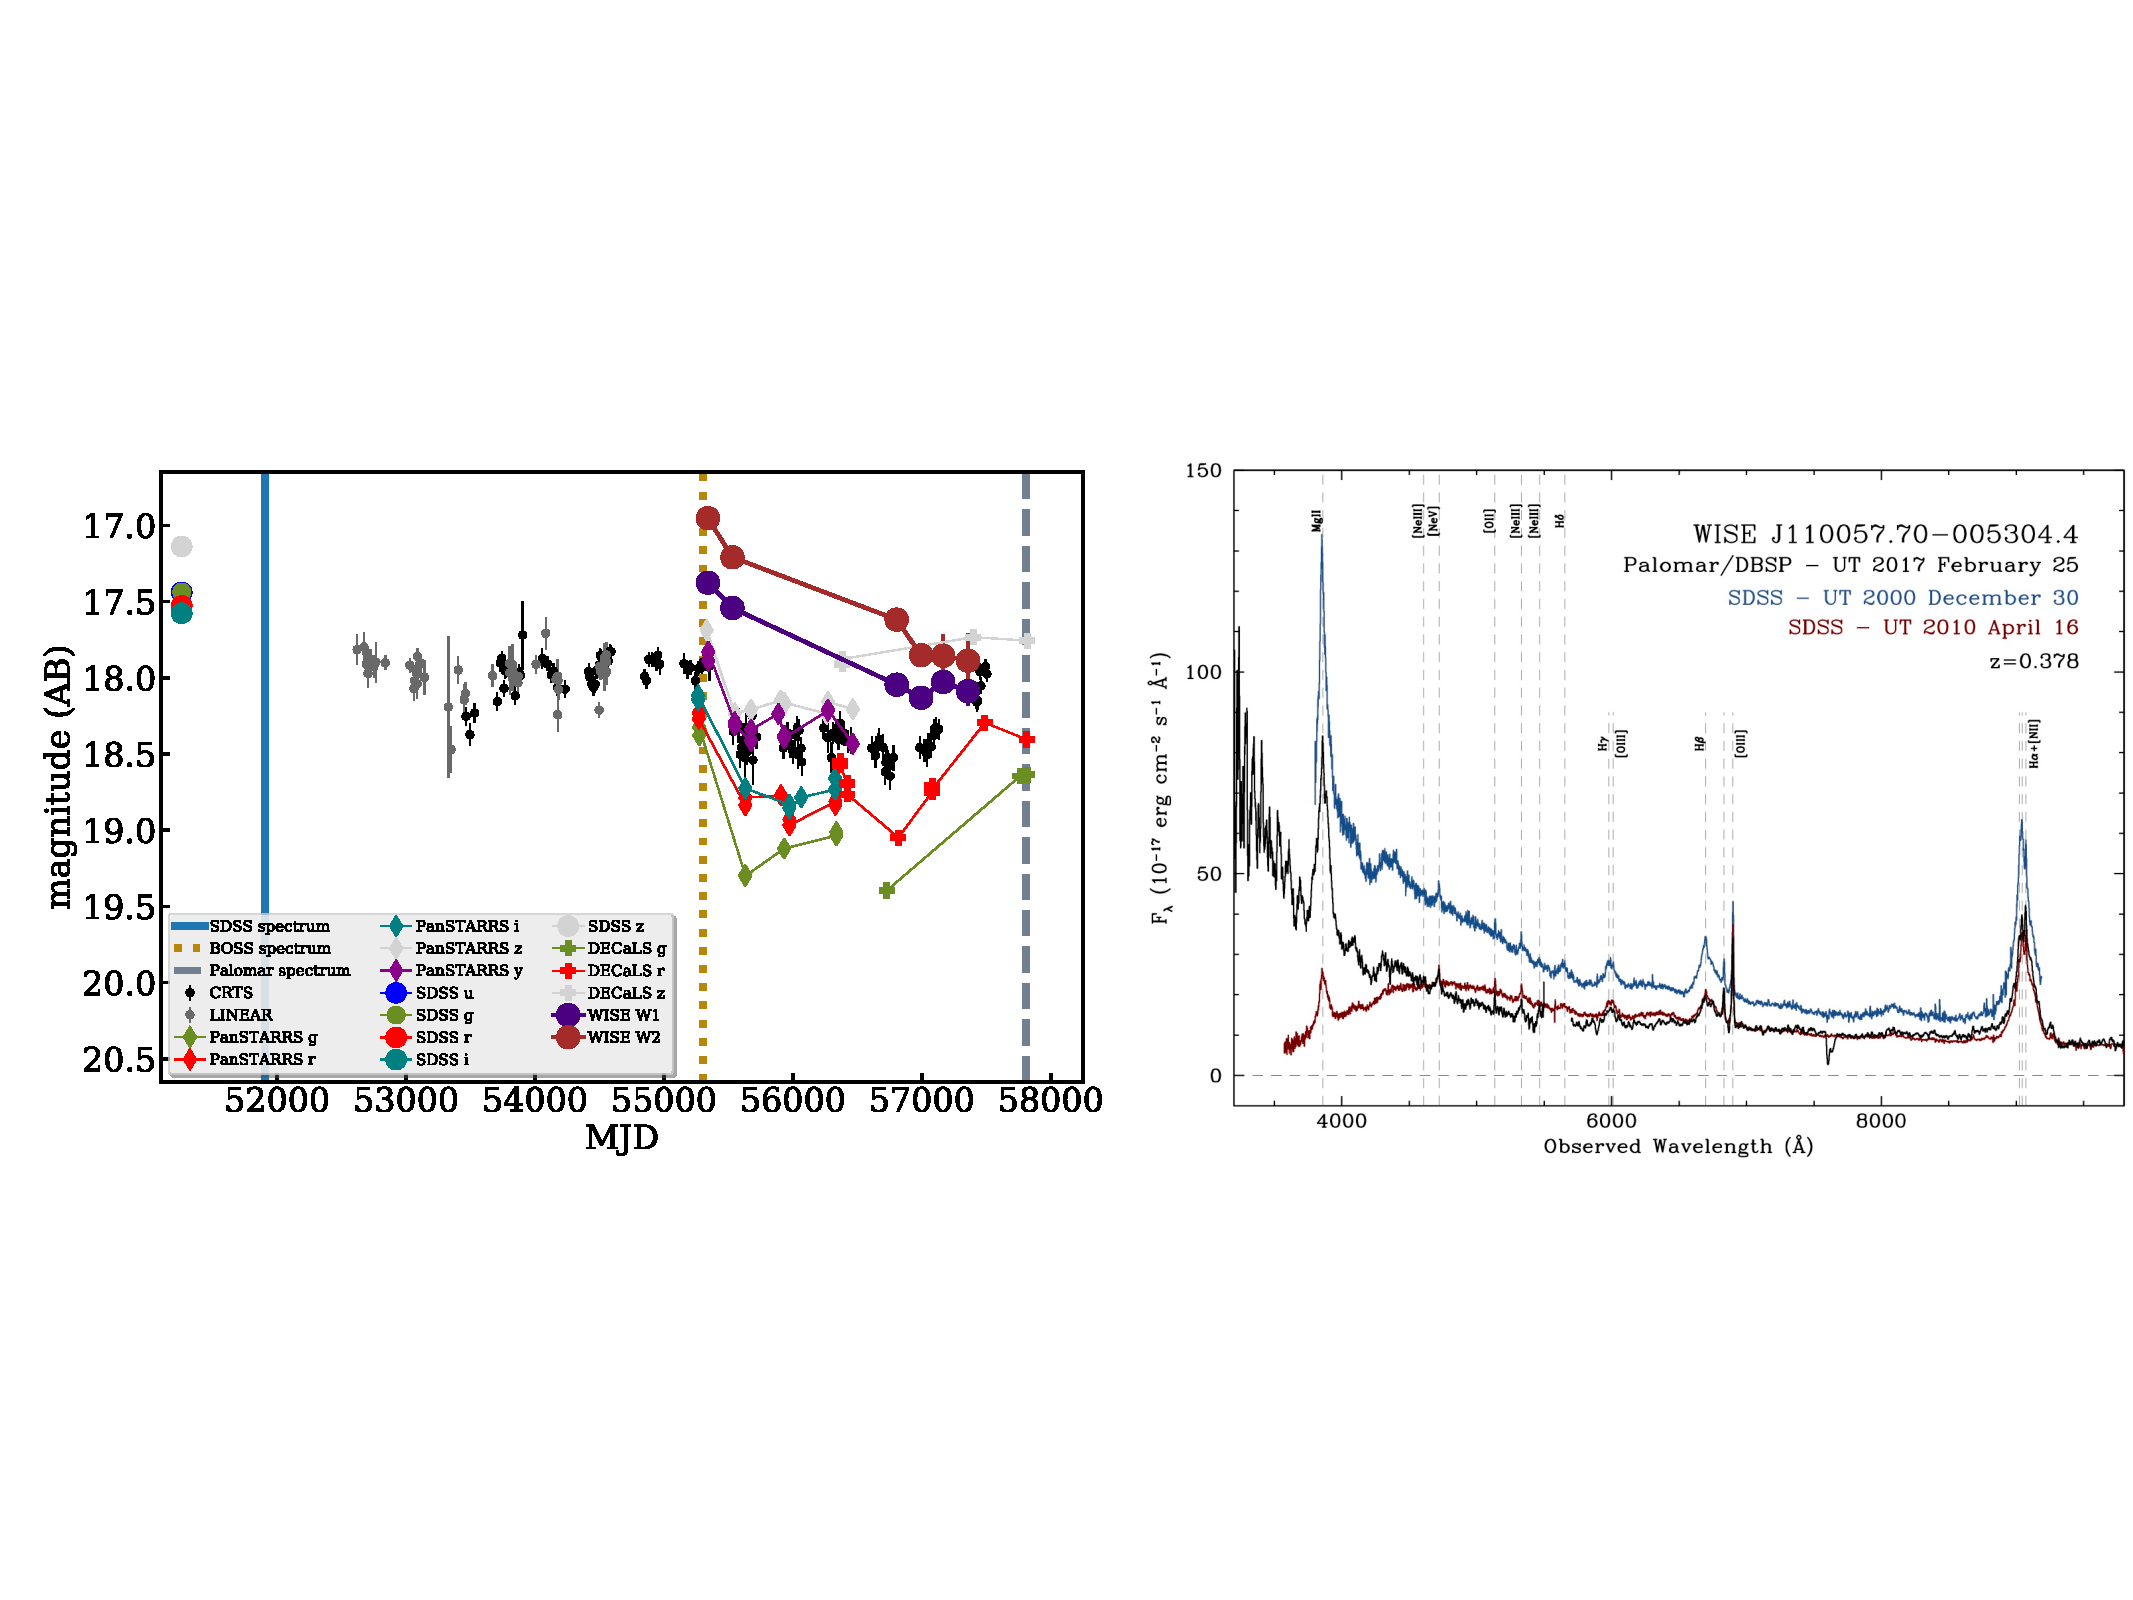
\includegraphics[height=6.25cm,width=17.2cm]
    {figures/J110057_LC_Spectra_20171024.pdf}
    \vspace{-10pt}
    \caption{\footnotesize 
      {\it (Left:)} The optical and infrared light-curve for
      J1100-0053; Note the fall in the infrared, whereas there is a
      decrease, but then recovery in the optical.  {\it (Right:)} Three
      epochs of spectra for J1100-0053.  The spectacular downturn in the
      blue for the 2010 spectrum indicates a dramatic change in the
      accretion disk.}
    \vspace{-16pt}
    \label{fig:J1100}
  \end{center}
\end{figure}

\smallskip
\smallskip
\noindent
\textbf{\textsc{New IR investigations into the CLQ Population:}}
Taking advantage of new optical imaging data from the Dark Energy
Camera Legacy Survey \href{http://legacysurvey.org/decamls/}{(DECaLS)}
and new IR light-curves from NEOWISE \citep{Meisner2017a,
Meisner2017b}, I have made further in-roads into understanding the CLQ
population. This includes identifying objects with rapidly changing IR
light-curves and also accretion disk changes, e.g. the $z=0.378$
quasar SDSS J110057-005304.4, see Figure~\ref{fig:J1100}. From
J1100-0053, my new model \citep{Ross2018} suggests a dramatic new
picture of the physics of the CLQs governed by processes at the
innermost stable circular orbit (ISCO) and the structure of the
innermost disk. Expanding these new observations in sample and
temporal size, in order to properly inform our theoretical
models is the next big challenge.

\smallskip
\smallskip
\noindent
{\bf In summary, as of the time of writing, the
observational state-of-the-art for extreme variable quasars is 44
objects, 11 of which I have either discovered or co-led the
discovery.}



\subsubsection{Theoretical State-of-the-Art}
Here we present a concise high-level overview of the theoretical
state-of-the-art and in particular focus on issues related to our
quasar studies.

\smallskip 
\smallskip
\noindent 
\textbf{\textsc{Contemporary Accretion Disk theory:}} 
The accretion disk scale is $\lesssim 10^{3}-10^{6}$ r$_{g}$, (where
$r_{\rm g}$ is the gravitational radius; $r_{\rm g}=\frac{GM}{c^2}$)
which, for a 10$^{8}$ M$_{\rm BH}$ is $\approx$5$\times$$10^{-3}$ to 5
pc.  \citet{YuanNarayan2014} review, black hole accretion flows can be
divided into two broad classes: cold and hot. Cold accretion flows
consist of cool optically thick gas and are found at relatively high
mass accretion rates.  Hot accretion flows, are virially hot and
optically thin, and occur at lower mass accretion rates.  How a
accretion disk flow transitions between `cold' and `hot', e.g. as the
mass flow rate $\dot{m}$ changes, is not well understood, and is an
area of current activity.


\smallskip 
\smallskip
\noindent 
\textbf{\textsc{Contemporary Galaxy formation theory:}}
Contemporary cosmological magnetohydrodynamical galaxy formation
simulations take into account a wide range of physical processes, use
state-of-the-art numerical codes and take weeks to months to run on
the largest supercomputers.  They are incredibly sophisticated
apparatus and allow us to gain deep insight into the physical
processes that drive galaxy formation, including the energy connected
to an accreting central SMBH. \citet{NaabOstriker2017} present an up
to date review of the major challenges for galaxy formation theory.

\smallskip 
\smallskip
\noindent 
Current state-of-the-art cosmological simulations, for example, the
EAGLE Project \citep{Schaye2015, Crain2015} and the IllustrisTNG
Project \citep{Pillepich2018} employ and track 10s of billions
resolution elements across 100s of megaparsec-cubed volumes.  For
EAGLE (e.g. their L100N1504 simulation), the fundamental units of
dimensions mass (M), length (L) and time (T, i.e. resolution) are
$\sim~2~\times10^{5}$ for initial baryonic particle mass, ``softening
lengths'' of 0.35-0.7 pkpc; and and time-steps sampling $\sim$1000
years ($\sim$10$^{6}$ time-steps across the age of the
Universe)\footnote{The times are spaced logarithmically in the
expansion factor $a$ such that $\Delta a = 0.005a$.}. For the new
IllustrisTNG ``TNG100'' model one has $1.4\times10^{6}$ for baryonic
particle mass, softening lengths $\approx$0.2-1 pkpc, and
$8\times10^{5} h^{-1}$ M$_{\odot}$ for the seed black hole mass.  As
such, these are extremely powerful for global galactic properties, but
these simulations cannot, and were never designed to, explicitly
address inner central engine physics.

\smallskip 
\smallskip
\noindent 
Further progress is made with the new high-resolution ``zoom-in''
galaxy simulations, e.g. Feedback In Realistic Environments
\citep[FIRE-2;][]{Wetzel2016, Hopkins2017} or MUFASA
\citep[][]{Dave2016}.  In FIRE-2 for example, \citet{Wetzel2016} run a
cosmological scale dark-matter-only simulation to redshift $z=0$. An
isolated DM halo is then selected, the particles are traced back to
very high, $z=100$ redshift and the `convex hull' is regenerated at
high resolution (embedded within the full lower-resolution volume).
The fiducial baryonic simulation contains dark matter, gas, and stars
within the zoom-in region, comprising 140 million total particles,
with $M_{\rm DM} =3.5\times10^{4} M_{\odot}$ and $M_{\rm gas,initial}
= 7070 M_{\odot}$.  The dark matter and stars have fixed gravitational
softening lengths of 20pc and 4pc, respectively.  In these zoom-ins,
the shortest time step achieved is 180 years.  As such, these
`zoom-in' simulations are impressive, but still not close enough to
resolving the scales, masses and cadences needed in order to
successful model e.g. the ``changing look'' quasars.

\smallskip 
\smallskip
\noindent 
However, what is remains very concerning is that even once the mass,
length and timescales are computationally accessible, {\it we
currently do not know what physical prescriptions should be directed
for the central black hole and quasar engines to follow.}

\smallskip
\smallskip
\noindent
For example and as described in detailed in \citet{Weinberger2017},
modelling AGNs in cosmological simulations poses several fundamental
challenges. The detailed physical mechanisms of both accretion on to
SMBHs, and the AGN-gas interaction are poorly understood
\citep{Hopkins_Quataert2010, Hopkins_Quataert2011,
Huarte-Espinosa2011, Gaibler2012, Angles-Alcazar2013, Gaspari2013,
Cielo2014, Costa2014, Angles-Alcazar2015, Emsellem2015,
CurtisSijacki2015, CurtisSijacki2016a, CurtisSijacki2016b,
Rosas-Guevara2015, Roos2015, Hopkins2016, Bieri2017,
Angles-Alcazar2017}. This makes it at present impossible to formulate
a `correct' treatment for simulations.  The long-time standard
physical mechanism of Bondi-Hoyle-Lyttleton accretion, i.e. that of
spherical accretion onto a compact object traveling through the
interstellar medium \citep{Hoyle_Lyttleton1939, Bondi_Hoyle1944,
Bondi1952} with the accretion rate given by $\dot {M}_{\rm Bondi} =
\pi G^{2 }M_{\rm BH}^{2} \, \rho / c_{s}^{3}$, {\it is known to
be a considerable oversimplification} \citep[e.g.,][]{Edgar2004}.
There is an urgent need for a new theory, and new observations will 
play a key role in guiding us and achieving this.




\smallskip
\smallskip
\noindent
{\bf \emph{The timing for this proposal could not be better or more imperative.} 
The first of the data ``firehoses'' turns on in late 2019, with
the full datastream from our key sources fully online around 2022. 
As such, with two years to use existing datasets as testbeds, we 
have the time to ramp-up our efforts, while also being able to 
take advantage of the initial data releases of all these new projects.}
%% LSST:: Each patch of sky it images will be visited 1000 times during the survey,


\subsection{Objectives}
%\smallskip \smallskip \noindent
%The outstanding issues and novel investigations that are pertinent to this proposal are summarised in the Table below. 

\smallskip
\smallskip
\noindent
The science questions we seek to address are well-posed, yet strike at the heart of major and still
open extragalactic astrophysical questions: 
\begin{itemize}
\item What is the main quasar triggering mechanism at the height of quasar activity? 
\item Do we have a full accounting of the accretion history in the Universe?   
\item What direct observational evidence links quasar activity to star formation?  
\item What are the star-formation properties of luminous quasars at the peak of quasar activity? 
\item How does the energy escape from the central engine and impact the host galaxy?  
\item Are the modes of AGN ``feedback'' that regulate the host galaxy the same that regulate the AGN itself?  
\item Can we observe ``quasar feedback'' in action, in situ, for the most luminous sources?   
\item What is the link between the observed properties of quasars, such as light curves and emission/absorption line spectra, 
and their underlying properties e.g., accretion rate, accretion disk structure and black hole mass and spin? 
\end{itemize}

\smallskip
\smallskip
\noindent
These questions have been raised for some time and are challenges
which need to be addressed now in order to make significant progress.


\smallskip
\smallskip
\noindent
Our ERC Consolidator grant proposal will radically improve our
understanding of one of the two fundamental energy sources available
to galaxies; that of accretion onto the compact object in the central
engine. We will achieve this by leveraging several of the new,
large-scale surveys that are coming online in the next few years.  The
scope and remit of an ERC Consolidator grant will allow us to combine
these data products in a manner that will not only establish the new
state-of-the-art in extragalactic variable astrophysics, {\it it will
establish and kick start the new field of extragalactic variable
astrophysics itself}.  The PI is a world-leader in observational quasar
astrophysics, both in terms of survey work and individual object
study.  Our proposal takes astrophysics into the 2020s, going from
single objects samples, to surveys and samples of millions of objects
leveraging these multi-billion \euro/\pounds/\$ next generation
missions, telescopes and their subsequent datasets.



\smallskip
\smallskip
\noindent
\textbf{\textsc{Maximising Science Returns from European priorities:}}
Contemporary astronomy is a multi-national endeavor with many leading
facilites being international collaborations. Although a project, with
similar but much less ambitious science goals and return could be
envisaged at the national level, the full discovery and break-through
nature being described herein only comes to the fore when the data
from the various international collaborations are combined
intelligently.  Critically data from leading European Southern
Observatory (ESO) and European Space Agency (ESA) facilities will play
a pivotal role here.

% At the end of this section you can include some sub headings on: \\

%Research Vision and aims
%Justification of why your vision and aims are important
%Where will your field be at the end of the funding period in terms of new knowledge? If you can explain this in some sort of schematic diagramme it would be even better.


\smallskip

